\documentclass[11pt]{article}

\usepackage{exscale}
\usepackage{graphicx}
\usepackage{amsmath}
\usepackage{latexsym}
\usepackage{times,mathptm}
\usepackage{epsfig}
\usepackage{tikz}

\textwidth 6.5truein          
\textheight 9.0truein
\oddsidemargin 0.0in
\topmargin -0.6in

\parindent 0pt          
%\parskip 5pt
%\def\baselinestretch{1.1}

\begin{document}

\begin{LARGE}
\centerline {\bf CSci 423 Homework 1}
\end{LARGE}
\vskip 0.25cm

\centerline{Due: 12:30 pm in class, Thursday, 9/12/19}
\centerline{Daniel Quiroga}

\begin{enumerate}

\item (5 points) Prove by induction that $2^n\ge n^2$, for integer $n\ge 4$.\newline 
Base case: $n = 4 ==>$ $2^{4} \geq 4^{2}$ check \newline
Induction step: Let $k \geq 4$ be given is true for $n = k$. Then \newline 
$2^{k+1} > (k+1)^{2} = k^2 + 2k + 1$ \newline 
$2^{k+1} = 2^k \times 2^1$ I assume that $2^k$ is $>$ $k^2$ \newline
$2^k \times 2^1 > k^2 \times 2 = 2k^2 > k^2 + 2k + 1$\newline 
Thus, holds for $n = k + 1$, and the proof of the induction step is complete. \newline 
Conclusion: By the principle of mathematical induction, it follows that $2^n\ge n^2$, is true for $n\ge 4$

Collaborators: NONE

\item (3, 3, 3 points) In class, we studied a DFA that accepts strings with $111$ as a substring. 
Here, give DFAs (in state diagrams, and each with no more than four states) that accept the following languages over the alphabet $\{0,1\}$:
\begin{enumerate}
\item The set of strings with $011$ as a substring
\begin{center}
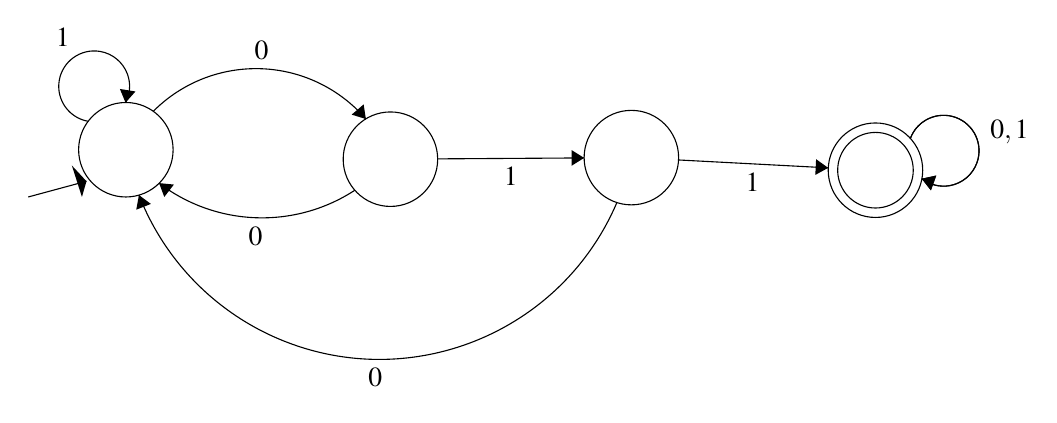
\begin{tikzpicture}[scale=0.2]
\tikzstyle{every node}+=[inner sep=0pt]
\draw [black] (1.8,-32) -- (5.5,-31);
\fill [black] (5.5,-31) -- (4.57,-30) -- (5.21,-32);
\draw [black] (8,-29) circle (3);
\draw [black] (24.8,-29.6) circle (3);
\draw [black] (40.1,-29.5) circle (3);
\draw [black] (55.6,-30.3) circle (3);
\draw [black] (55.6,-30.3) circle (2.4);
\draw [black] (9.733,-26.568) arc (135.18958:40.7196:9.208);
\fill [black] (23.24,-27.05) -- (23.1,-26.12) -- (22.34,-26.77);
\draw (16.62,-23.32) node [above] {$0$};
\draw [black] (27.8,-29.58) -- (37.1,-29.52);
\fill [black] (37.1,-29.52) -- (36.3,-29.02) -- (36.3,-30.02);
\draw (32.45,-30.06) node [below] {$1$};
\draw [black] (43.1,-29.65) -- (52.6,-30.15);
\fill [black] (52.6,-30.15) -- (51.83,-29.6) -- (51.78,-30.6);
\draw (47.8,-30.45) node [below] {$1$};
\draw [black] (57.813,-28.292) arc (159.9454:-128.0546:2.25);
\draw (62.86,-27.88) node [right] {$0,1$};
\fill [black] (58.54,-30.84) -- (59.12,-31.58) -- (59.46,-30.64);
\draw [black] (57.813,-28.292) arc (159.9454:-128.0546:2.25);
\fill [black] (58.54,-30.84) -- (59.12,-31.58) -- (59.46,-30.64);
\draw [black] (22.548,-31.567) arc (-56.83408:-127.25673:10.795);
\fill [black] (10.11,-31.12) -- (10.44,-32) -- (11.05,-31.21);
\draw (16.23,-33.85) node [below] {$0$};
\draw [black] (39.181,-32.351) arc (-23.11044:-158.67433:16.395);
\fill [black] (8.83,-31.88) -- (8.66,-32.81) -- (9.59,-32.44);
\draw (23.84,-42.82) node [below] {$0$};
\draw [black] (5.619,-27.195) arc (260.56505:-27.43495:2.25);
\draw (3.99,-22.46) node [above] {$1$};
\fill [black] (7.98,-26.01) -- (8.61,-25.3) -- (7.62,-25.14);
\end{tikzpicture}
\end{center}
\item The set of strings with $110$ as a substring
\begin{center}
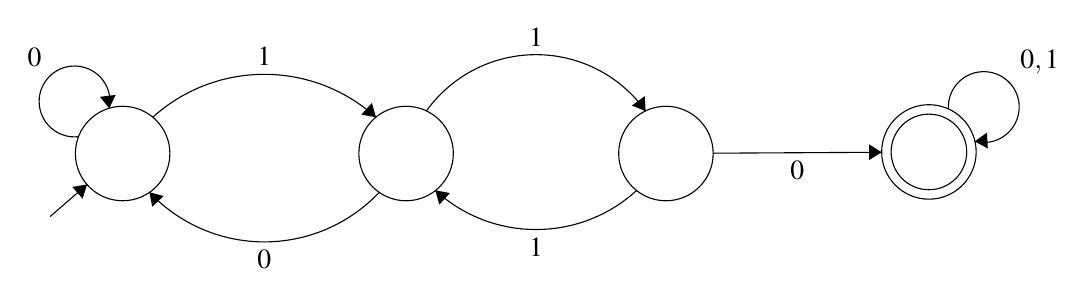
\begin{tikzpicture}[scale=0.2]
\tikzstyle{every node}+=[inner sep=0pt]
\draw [black] (13.8,-27.9) circle (3);
\draw [black] (31.8,-27.9) circle (3);
\draw [black] (48.3,-27.9) circle (3);
\draw [black] (65,-27.8) circle (3);
\draw [black] (65,-27.8) circle (2.4);
\draw [black] (9.2,-31.9) -- (11.54,-29.87);
\fill [black] (11.54,-29.87) -- (10.6,-30.02) -- (11.26,-30.77);
\draw [black] (11.011,-26.828) arc (276.70939:-11.29061:2.25);
\draw (8.21,-22.45) node [above] {$0$};
\fill [black] (12.95,-25.03) -- (13.36,-24.18) -- (12.36,-24.3);
\draw [black] (15.711,-25.601) arc (132.12884:47.87116:10.567);
\fill [black] (29.89,-25.6) -- (29.63,-24.69) -- (28.96,-25.43);
\draw (22.8,-22.37) node [above] {$1$};
\draw [black] (30.099,-30.358) arc (-43.25442:-136.74558:10.022);
\fill [black] (15.5,-30.36) -- (15.68,-31.28) -- (16.41,-30.6);
\draw (22.8,-34.01) node [below] {$0$};
\draw [black] (33.085,-25.206) arc (144.45594:35.54406:8.56);
\fill [black] (47.01,-25.21) -- (46.96,-24.26) -- (46.14,-24.85);
\draw (40.05,-21.12) node [above] {$1$};
\draw [black] (51.3,-27.88) -- (62,-27.82);
\fill [black] (62,-27.82) -- (61.2,-27.32) -- (61.2,-28.32);
\draw (56.65,-28.36) node [below] {$0$};
\draw [black] (46.444,-30.241) arc (-47.49295:-132.50705:9.463);
\fill [black] (33.66,-30.24) -- (33.91,-31.15) -- (34.58,-30.41);
\draw (40.05,-33.23) node [below] {$1$};
\draw [black] (66.237,-25.08) arc (183.28941:-104.71059:2.25);
\draw (70.78,-22.09) node [right] {$0,1$};
\fill [black] (67.91,-27.13) -- (68.74,-27.58) -- (68.68,-26.58);
\end{tikzpicture}
\end{center}
\item The set of strings with $101$ as a substring
\begin{center}
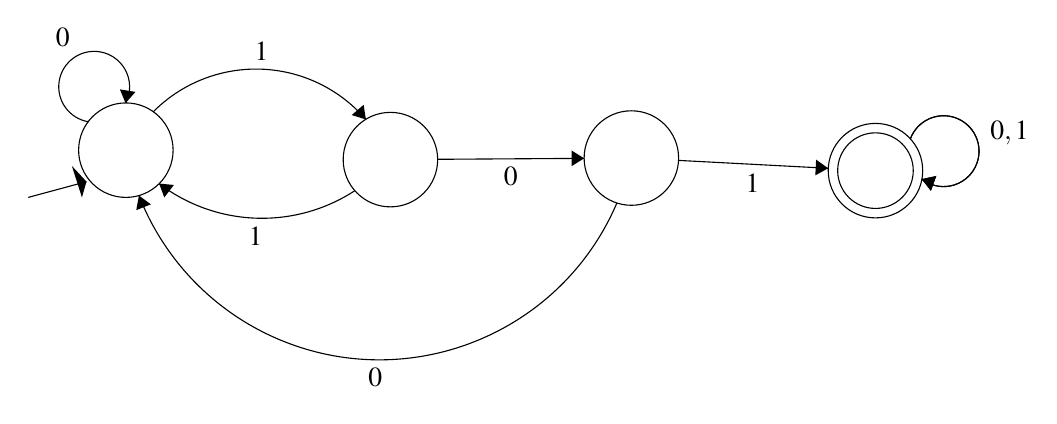
\begin{tikzpicture}[scale=0.2]
\tikzstyle{every node}+=[inner sep=0pt]
\draw [black] (1.8,-32) -- (5.5,-31);
\fill [black] (5.5,-31) -- (4.57,-30) -- (5.21,-32);
\draw [black] (8,-29) circle (3);
\draw [black] (24.8,-29.6) circle (3);
\draw [black] (40.1,-29.5) circle (3);
\draw [black] (55.6,-30.3) circle (3);
\draw [black] (55.6,-30.3) circle (2.4);
\draw [black] (9.733,-26.568) arc (135.18958:40.7196:9.208);
\fill [black] (23.24,-27.05) -- (23.1,-26.12) -- (22.34,-26.77);
\draw (16.62,-23.32) node [above] {$1$};
\draw [black] (27.8,-29.58) -- (37.1,-29.52);
\fill [black] (37.1,-29.52) -- (36.3,-29.02) -- (36.3,-30.02);
\draw (32.45,-30.06) node [below] {$0$};
\draw [black] (43.1,-29.65) -- (52.6,-30.15);
\fill [black] (52.6,-30.15) -- (51.83,-29.6) -- (51.78,-30.6);
\draw (47.8,-30.45) node [below] {$1$};
\draw [black] (57.813,-28.292) arc (159.9454:-128.0546:2.25);
\draw (62.86,-27.88) node [right] {$0,1$};
\fill [black] (58.54,-30.84) -- (59.12,-31.58) -- (59.46,-30.64);
\draw [black] (57.813,-28.292) arc (159.9454:-128.0546:2.25);
\fill [black] (58.54,-30.84) -- (59.12,-31.58) -- (59.46,-30.64);
\draw [black] (22.548,-31.567) arc (-56.83408:-127.25673:10.795);
\fill [black] (10.11,-31.12) -- (10.44,-32) -- (11.05,-31.21);
\draw (16.23,-33.85) node [below] {$1$};
\draw [black] (39.181,-32.351) arc (-23.11044:-158.67433:16.395);
\fill [black] (8.83,-31.88) -- (8.66,-32.81) -- (9.59,-32.44);
\draw (23.84,-42.82) node [below] {$0$};
\draw [black] (5.619,-27.195) arc (260.56505:-27.43495:2.25);
\draw (3.99,-22.46) node [above] {$0$};
\fill [black] (7.98,-26.01) -- (8.61,-25.3) -- (7.62,-25.14);
\end{tikzpicture}
\end{center}
\end{enumerate}

Collaborators: NONE

\item (5 points) Give the state diagram of a DFA with no more than 12 states that accepts the language containing
all strings in $\{0,1\}^*$ such that in each string the number of 0s is divisible by 4 and the number of 1s is divisible by 3.


Daniel Quiroga <dquiroga@email.wm.edu>
9:42 PM (0 minutes ago)

to me

\begin{center}
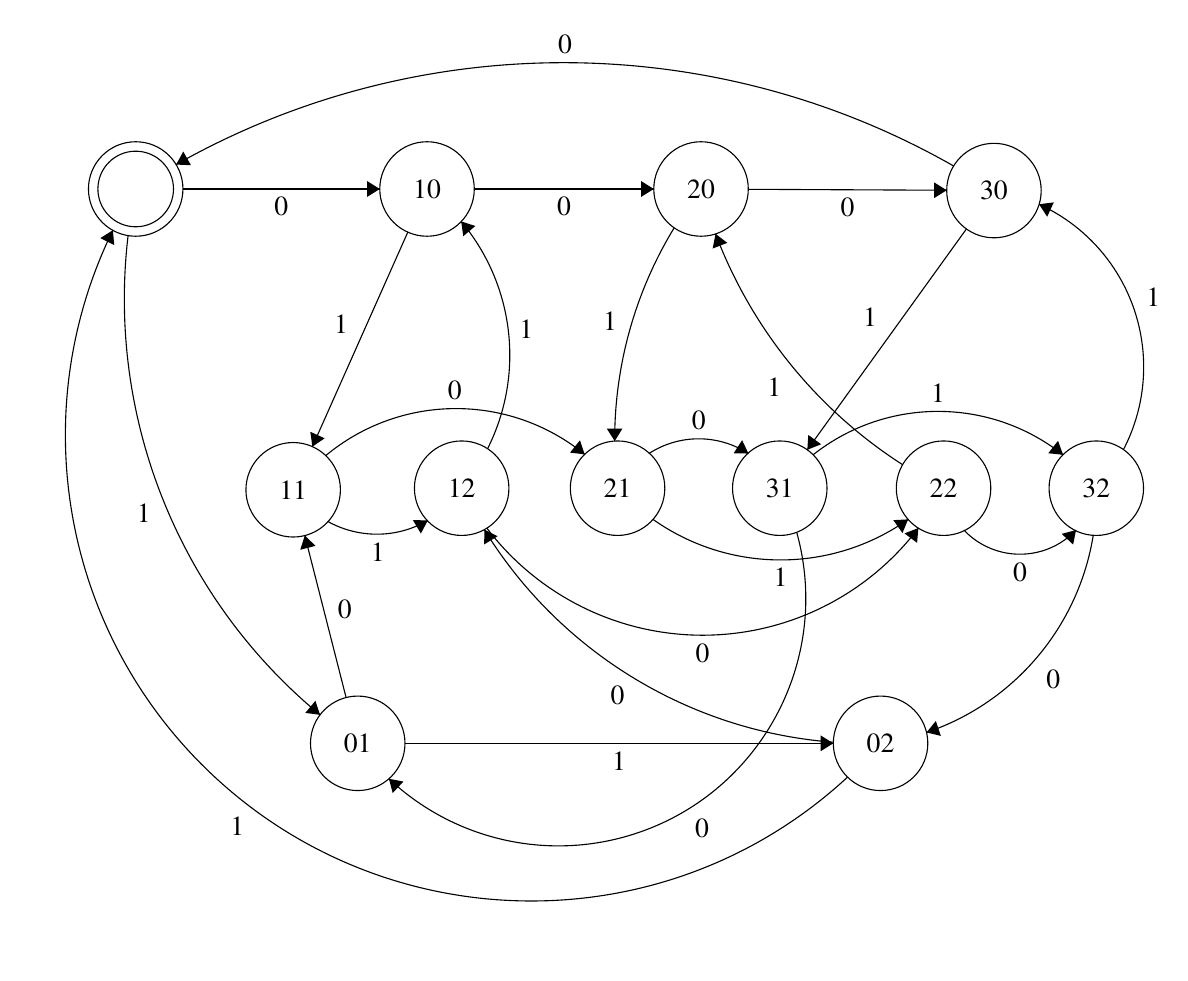
\begin{tikzpicture}[scale=0.2]
\tikzstyle{every node}+=[inner sep=0pt]
\draw [black] (11.1,-12.9) circle (3);
\draw [black] (11.1,-12.9) circle (2.4);
\draw [black] (29.6,-12.9) circle (3);
\draw (29.6,-12.9) node {$10$};
\draw [black] (47,-12.9) circle (3);
\draw (47,-12.9) node {$20$};
\draw [black] (65.6,-13) circle (3);
\draw (65.6,-13) node {$30$};
\draw [black] (25.2,-48.1) circle (3);
\draw (25.2,-48.1) node {$01$};
\draw [black] (58.4,-48.1) circle (3);
\draw (58.4,-48.1) node {$02$};
\draw [black] (21.1,-32) circle (3);
\draw (21.1,-32) node {$11$};
\draw [black] (31.8,-31.9) circle (3);
\draw (31.8,-31.9) node {$12$};
\draw [black] (41.7,-31.9) circle (3);
\draw (41.7,-31.9) node {$21$};
\draw [black] (52,-31.9) circle (3);
\draw (52,-31.9) node {$31$};
\draw [black] (62.4,-31.9) circle (3);
\draw (62.4,-31.9) node {$22$};
\draw [black] (72.1,-31.9) circle (3);
\draw (72.1,-31.9) node {$32$};
\draw [black] (14.1,-12.9) -- (26.6,-12.9);
\fill [black] (26.6,-12.9) -- (25.8,-12.4) -- (25.8,-13.4);
\draw (20.35,-13.4) node [below] {$0$};
\draw [black] (22.807,-46.292) arc (-129.58477:-186.7563:34.258);
\fill [black] (22.81,-46.29) -- (22.51,-45.4) -- (21.87,-46.17);
\draw (12.09,-33.51) node [left] {$1$};
\draw [black] (28.38,-15.64) -- (22.32,-29.26);
\fill [black] (22.32,-29.26) -- (23.1,-28.73) -- (22.19,-28.32);
\draw (24.62,-21.46) node [left] {$1$};
\draw [black] (24.46,-45.19) -- (21.84,-34.91);
\fill [black] (21.84,-34.91) -- (21.55,-35.81) -- (22.52,-35.56);
\draw (23.91,-39.58) node [right] {$0$};
\draw [black] (28.2,-48.1) -- (55.4,-48.1);
\fill [black] (55.4,-48.1) -- (54.6,-47.6) -- (54.6,-48.6);
\draw (41.8,-48.6) node [below] {$1$};
\draw [black] (55.402,-48.03) arc (-94.346:-148.33872:28.585);
\fill [black] (33.24,-34.53) -- (33.23,-35.47) -- (34.08,-34.95);
\draw (41.7,-44.44) node [below] {$0$};
\draw [black] (56.305,-50.245) arc (-47.22603:-206.08619:29.582);
\fill [black] (9.65,-15.52) -- (8.85,-16.02) -- (9.74,-16.46);
\draw (17.55,-52.76) node [below] {$1$};
\draw [black] (32.6,-12.9) -- (44,-12.9);
\fill [black] (44,-12.9) -- (43.2,-12.4) -- (43.2,-13.4);
\draw (38.3,-13.4) node [below] {$0$};
\draw [black] (50,-12.92) -- (62.6,-12.98);
\fill [black] (62.6,-12.98) -- (61.8,-12.48) -- (61.8,-13.48);
\draw (56.3,-13.46) node [below] {$0$};
\draw [black] (41.516,-28.907) arc (-179.80363:-211.36898:25.845);
\fill [black] (41.52,-28.91) -- (42.01,-28.11) -- (41.01,-28.11);
\draw (41.7,-21.33) node [left] {$1$};
\draw [black] (63.85,-15.44) -- (53.75,-29.46);
\fill [black] (53.75,-29.46) -- (54.63,-29.11) -- (53.81,-28.52);
\draw (58.21,-21.07) node [left] {$1$};
\draw [black] (13.666,-11.347) arc (119.45948:60.33026:50.033);
\fill [black] (13.67,-11.35) -- (14.61,-11.39) -- (14.12,-10.52);
\draw (38.36,-4.38) node [above] {$0$};
\draw [black] (29.647,-33.949) arc (-59.80197:-119.12711:6.421);
\fill [black] (29.65,-33.95) -- (28.7,-33.92) -- (29.21,-34.78);
\draw (26.48,-35.33) node [below] {$1$};
\draw [black] (23.165,-29.833) arc (129.73424:50.82202:12.942);
\fill [black] (39.61,-29.75) -- (39.31,-28.86) -- (38.68,-29.64);
\draw (31.37,-26.34) node [above] {$0$};
\draw [black] (60.803,-34.435) arc (-37.2118:-142.7882:17.206);
\fill [black] (60.8,-34.43) -- (59.92,-34.77) -- (60.72,-35.37);
\draw (47.1,-41.74) node [below] {$0$};
\draw [black] (31.77,-14.962) arc (39.96608:-26.75641:13.213);
\fill [black] (31.77,-14.96) -- (31.9,-15.9) -- (32.67,-15.25);
\draw (35.43,-21.81) node [right] {$1$};
\draw [black] (43.69,-29.7) arc (123.03128:56.96872:5.796);
\fill [black] (50.01,-29.7) -- (49.61,-28.85) -- (49.07,-29.68);
\draw (46.85,-28.26) node [above] {$0$};
\draw [black] (60.154,-33.88) arc (-54.72689:-125.27311:14.033);
\fill [black] (60.15,-33.88) -- (59.21,-33.93) -- (59.79,-34.75);
\draw (52.05,-36.96) node [below] {$1$};
\draw [black] (53.074,-34.696) arc (15.538:-133.23396:15.71);
\fill [black] (27.18,-50.35) -- (27.42,-51.26) -- (28.1,-50.53);
\draw (47.06,-52.85) node [below] {$0$};
\draw [black] (54.114,-29.781) arc (128.33918:51.66082:12.793);
\fill [black] (69.99,-29.78) -- (69.67,-28.89) -- (69.05,-29.68);
\draw (62.05,-26.52) node [above] {$1$};
\draw [black] (70.812,-34.558) arc (-43.37999:-136.62001:4.901);
\fill [black] (70.81,-34.56) -- (69.9,-34.8) -- (70.63,-35.48);
\draw (67.25,-36.59) node [below] {$0$};
\draw [black] (59.799,-30.407) arc (-122.71473:-159.23392:30.101);
\fill [black] (47.92,-15.75) -- (47.74,-16.68) -- (48.67,-16.32);
\draw (52.12,-25.46) node [left] {$1$};
\draw [black] (68.462,-13.871) arc (65.49916:-27.5414:11.354);
\fill [black] (68.46,-13.87) -- (68.98,-14.66) -- (69.4,-13.75);
\draw (75.25,-19.78) node [right] {$1$};
\draw [black] (71.905,-34.889) arc (-9.15084:-71.29016:15.888);
\fill [black] (61.32,-47.41) -- (62.23,-47.63) -- (61.91,-46.68);
\draw (68.9,-44.06) node [right] {$0$};
\end{tikzpicture}
\end{center}


\item (3 points) Assume language $A$ is accepted by DFA $M$. Describe a simple method in just one short sentence to construct a DFA $\overline{M}$ that accepts $\overline A$.

$\bar{M} = \{ v \* \| v \notin A \}$ would give you a DFA $\bar{M}$ that accepts all of $\bar{A}$

Collaborators: Yang Zhang

\item (4, 4 points) For the following DFAs given in the transition table format, draw their state diagrams and then describe precisely and concisely 
the languages accepted by the DFAs.
\begin{enumerate}

\item

\begin{tabular}{r||c|c}
& 0 & 1 \\\hline\hline
$\rightarrow$ $q_0$ & $q_1$ & $q_0$ \\\hline
*$q_1$ & $q_2$ & $q_0$ \\\hline
$q_2$ & $q_2$ & $q_2$ \\
\end{tabular}

$L_1=\{w\in\{0,1\}^* | w{\rm \ ends\ with\ a \ 0\ and\ doesn't\ have \ substring\  00}\}$

\begin{center}
\begin{tikzpicture}[scale=0.2]
\tikzstyle{every node}+=[inner sep=0pt]
\draw [black] (13.9,-19.7) circle (3);
\draw (13.9,-19.7) node {$q_0$};
\draw [black] (50.6,-19.9) circle (3);
\draw (50.6,-19.9) node {$q_1$};
\draw [black] (50.6,-19.9) circle (2.4);
\draw [black] (32.2,-39.8) circle (3);
\draw (32.2,-39.8) node {$q_2$};
\draw [black] (16.554,-18.303) arc (115.38134:63.99419:36.221);
\fill [black] (47.96,-18.47) -- (47.46,-17.67) -- (47.02,-18.57);
\draw (32.28,-14.3) node [above] {$0$};
\draw [black] (12.577,-17.02) arc (234:-54:2.25);
\draw (13.9,-12.45) node [above] {$1$};
\fill [black] (15.22,-17.02) -- (16.1,-16.67) -- (15.29,-16.08);
\draw [black] (48.029,-21.444) arc (-61.62625:-118.99822:32.891);
\fill [black] (16.45,-21.27) -- (16.91,-22.1) -- (17.4,-21.22);
\draw (32.22,-25.9) node [below] {$1$};
\draw [black] (50.316,-22.884) arc (-9.63421:-75.88017:20.438);
\fill [black] (35.15,-39.28) -- (36.05,-39.57) -- (35.81,-38.6);
\draw (45.71,-34.8) node [right] {$0$};
\draw [black] (33.523,-42.48) arc (54:-234:2.25);
\draw (32.2,-47.05) node [below] {$0,1$};
\fill [black] (30.88,-42.48) -- (30,-42.83) -- (30.81,-43.42);
\draw [black] (7.9,-27.7) -- (12.1,-22.1);
\fill [black] (12.1,-22.1) -- (11.22,-22.44) -- (12.02,-23.04);
\end{tikzpicture}
\end{center}

\item
\begin{tabular}{r||c|c}
& 0 & 1\\\hline
$\rightarrow$*$q_0$ & $q_1$ & $q_2$ \\\hline
*$q_1$ & $q_3$ & $q_2$ \\\hline
*$q_2$ & $q_1$ & $q_3$ \\\hline
$q_3$ & $q_3$ & $q_3$ \\
\end{tabular}

$L_2=\{w\in\{0,1\}^* | w{\rm\ doesn't\ contain\ substrings\  00\ or\ 11}\}$

\begin{center}
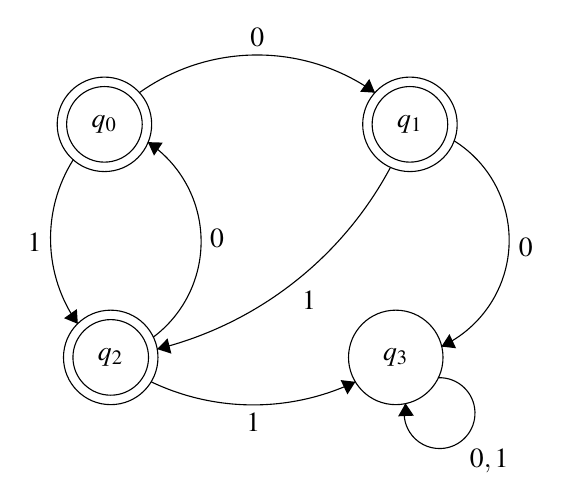
\begin{tikzpicture}[scale=0.2]
\tikzstyle{every node}+=[inner sep=0pt]
\draw [black] (11.7,-17.2) circle (3);
\draw (11.7,-17.2) node {$q_0$};
\draw [black] (11.7,-17.2) circle (2.4);
\draw [black] (31.1,-17.2) circle (3);
\draw (31.1,-17.2) node {$q_1$};
\draw [black] (31.1,-17.2) circle (2.4);
\draw [black] (12.1,-32) circle (3);
\draw (12.1,-32) node {$q_2$};
\draw [black] (12.1,-32) circle (2.4);
\draw [black] (30.2,-32) circle (3);
\draw (30.2,-32) node {$q_3$};
\draw [black] (13.918,-15.19) arc (125.50095:54.49905:12.883);
\fill [black] (28.88,-15.19) -- (28.52,-14.32) -- (27.94,-15.13);
\draw (21.4,-12.3) node [above] {$0$};
\draw [black] (10.006,-29.87) arc (-144.65244:-212.25125:9.378);
\fill [black] (10.01,-29.87) -- (9.95,-28.93) -- (9.14,-29.51);
\draw (7.74,-24.7) node [left] {$1$};
\draw [black] (14.457,-18.331) arc (56.35945:-53.26314:7.583);
\fill [black] (14.46,-18.33) -- (14.85,-19.19) -- (15.4,-18.36);
\draw (18.38,-24.43) node [right] {$0$};
\draw [black] (29.864,-19.931) arc (-28.07255:-76.09402:23.073);
\fill [black] (15.05,-31.47) -- (15.95,-31.76) -- (15.71,-30.79);
\draw (24.69,-27.77) node [below] {$1$};
\draw [black] (33.893,-18.238) arc (58.07158:-65.03141:7.446);
\fill [black] (33.1,-31.31) -- (34.03,-31.42) -- (33.61,-30.52);
\draw (37.98,-25.04) node [right] {$0$};
\draw [black] (27.638,-33.55) arc (-64.52196:-115.47804:15.081);
\fill [black] (27.64,-33.55) -- (26.7,-33.44) -- (27.13,-34.35);
\draw (21.15,-35.52) node [below] {$1$};
\draw [black] (32.896,-33.29) arc (92.15723:-195.84277:2.25);
\draw (36.13,-37.8) node [below] {$0,1$};
\fill [black] (30.82,-34.92) -- (30.35,-35.74) -- (31.35,-35.7);
\end{tikzpicture}
\end{center}

\end{enumerate}

Collaborators: Yang Zhang

\end{enumerate}

\end{document}